\NewDocumentCommand\RQ{+m}{{\bf RQ$_{#1}$}}

\chapter{Introduction}
\label{ch:intro}

% \begin{abstract}
% Sample Abstract.
% \end{abstract}

Software engineering, a cornerstone of modern technological advancement, plays a pivotal role in shaping society. It involves the systematic application of engineering principles to the design, development, testing, and maintenance of software~\cite{ianbook}. This discipline not only focuses on functionality and performance but also on ensuring the reliability and security of software systems. As a result, software engineers have created complex systems that power everything from global communication networks and financial systems to personal computing devices and medical equipment~\cite{ke2012software, rausch2013software}.

The impact of software engineering on society is profound and multifaceted. It has drastically transformed how we work, communicate, and live, making processes more efficient and information more accessible~\cite{ianbook}. Innovations such as the internet, mobile applications, and cloud computing, all software engineering products, have revolutionized industries such as
computer games, music, and film and television~\cite{vaudour2020software}. Moreover, these advances have democratized access to information, connected global communities, and facilitated advancements in other fields such as healthcare, education, and transportation~\cite{xu2018industry}.

Building on the foundational aspects of software engineering, software analysis is a critical component that ensures software systems are efficient, secure, and error-free. This analytical process includes analyses such as type inference and call graph construction, which help optimize code and enhance its performance~\cite{nielson2015principles}. Type inference automatically determines the types of expressions in a programming language without explicit type annotations, simplifying code maintenance and improving readability. Call graph construction, meanwhile, focuses on finding all possible function calls within a program, providing a visual and analytical map that developers use to optimize execution paths and enhance performance~\cite{ryder1979constructing}.

The actionability of software analysis tools is a critical factor influencing their adoption and effectiveness in software development. Actionability refers to the tool's ability to provide developers with clear, practical steps to resolve detected issues. This is vital because actionable warnings help developers quickly understand and address problems, thus enhancing productivity and code quality. Conversely, false warnings, or false positives, are instances where the tool incorrectly flags non-issues as problems. High rates of false positives can lead to "alert fatigue," where developers become desensitized to warnings and may start ignoring or turning off the analysis tools altogether. Minimizing false warnings and maximizing actionability are prominent. Tools that produce too many false positives are seen as unreliable and can erode trust among developers, leading to decreased usage and effectiveness. On the other hand, tools with high actionability support developers in maintaining and improving code quality. Balancing these factors is crucial for the practical adoption of static analysis tools in real-world software development environments~\cite{christakis2016developers, johnson2013don}.

Scalability is a significant problem in software analysis due to large-scale software systems' increasing complexity and resource demands. Larger codebases mean more lines of code, more functions, and more intricate interdependencies to analyze, all requiring considerable processing power and time. Also, maintaining up-to-date analysis in the face of frequent incremental changes, such as new features and bug fixes, poses another scalability challenge. Ensuring accurate analysis without reprocessing the entire codebase necessitates sophisticated techniques for partial analysis and data caching. Balancing precision and performance becomes increasingly difficult as more detailed analyses demand significant computation. 

Recently, machine learning has shown impressive performance in tackling various tasks in software analysis, particularly those involving the examination and manipulation of source code. Over recent years, the use of ML techniques for software analysis tasks has expanded and diversified significantly. These tasks include but are not limited to automated testing, bug detection, source code summarization, program repair, and type inference~\cite{sharma2024}. The success of ML in software analysis largely derives from its ability to learn from vast datasets of source code, which subsequently facilitates the automation of traditionally manual and error-prone tasks. For instance, ML methods have been applied to enhance software testing by automating the generation of test cases and optimizing testing workflows~\cite{schafer2023empirical}. Additionally, in the area of program repair, ML models are trained to predict and rectify bugs automatically, significantly reducing the manual effort required in debugging.

A key advantage of ML in this domain is its ability to provide actionable predictions that directly aid developers. For instance, in bug detection, ML models can be trained on large codebases to learn patterns associated with common bugs. When analyzing a new program, these models do not just flag potential issues but can pinpoint specific lines or methods likely containing bugs or vulnerabilities~\cite {fu2022linevul}, offering developers concrete starting points for debugging. Similarly, in program repair tasks, ML models trained on pairs of buggy and corrected code can suggest exact changes, such as modifying a condition in an if-statement or adding a null check—providing developers with ready-to-implement fixes~\cite{zhang2023survey}.

Moreover, ML models scale better with the size and complexity of programs. As mentioned, traditional static analysis tools often struggle with large codebases, as their rule-based approaches lead to exponential growth in analysis time or a surge in false positives. In contrast, ML models, particularly those based on deep learning architectures like transformers, excel at capturing long-range dependencies in code~\cite{maunveiling}. When trained on diverse, large-scale datasets, these models learn hierarchical representations, from token-level patterns to class-level structures, enabling them to understand the context of a given code snippet within its broader class or module. This hierarchical learning allows ML models to maintain high accuracy even when analyzing large programs. 

In this thesis, we aim to improve the actionability and scalability of software analysis by leveraging the power of machine learning. Our primary focus is on addressing two significant challenges: improving type inference for Python and refining call graph construction. These areas present substantial uncertainty, particularly in the realms of predicting type annotations accurately and constructing call graphs precisely. Python's dynamic nature and flexibility can lead to ambiguous type information, making traditional static analysis methods less effective. This ambiguity can cause issues such as missed type errors and less efficient code analysis, ultimately impacting code quality. To mitigate these uncertainties, we seek to explore ML-based techniques to predict type annotations in Python code. Machine learning models can learn from vast amounts of code corpus to identify patterns and infer types more accurately than traditional heuristic-based methods. By doing so, we aim to improve code quality, reduce runtime errors, and enhance the developer experience through more accurate code analysis and features like auto-completion.

Similarly, call graph construction faces challenges due to dynamic method calls and runtime behavior that static analysis may over-approximate. Traditional static analysis can result in call graphs with unnecessary or false edges, leading to false positives and reduced trust in the analysis tools. We propose employing machine learning models to analyze dynamic traces from program executions. By integrating insights from these dynamic traces, we can refine static call graphs, pruning unnecessary or false edges, and thereby reducing false positives. Our approach aims to align with developer preferences for fewer false alerts, increasing the trust and reliance on software analysis tools. We anticipate that enhancing the precision of call graphs will positively impact various downstream analyses, such as security assessments, making them more efficient and actionable. Machine learning offers a promising solution to handle the inherent uncertainties in software analysis, providing a more robust and scalable approach to improving type inference and call graph construction.

Additionally, we explore the application of call graphs in vulnerability analysis. Our approach involves adopting a granular methodology to identify at-risk Maven packages accurately, demonstrating that the value of granular vulnerability assessments over simpler, dependency-level analyses. Through this work, we aim to highlight the value of fine-grained vulnerability assessments in offering actionable insights for improving security practices in software development. Overall, this thesis aspires to push the boundaries of software analysis by developing powerful, ML-driven tools. These tools are intended to empower developers to build robust, secure, and maintainable software systems, addressing the pressing challenges of modern software development with promising solutions.

\section{Background}
Software analysis is a critical phase in the software development lifecycle that involves examining and evaluating a software product to understand its structure, functionality, and behavior. This process is essential for identifying potential issues, ensuring compliance with specifications, and verifying that the software meets its intended objectives. Software analysis can be divided into various forms, including static, dynamic, and formal methods, each serving unique purposes and providing different insights into the software system.

Static analysis refers to examining the software's behavior without executing the program. This type of analysis is conducted using tools that inspect the source code to detect possible vulnerabilities, coding errors, and style issues. It is beneficial for finding syntax errors, type mismatches, and other anomalies that could lead to software failure, all of which can be identified without running the program. Static analysis tools automate much of the review process, enabling developers to identify issues early in the development cycle. This not only helps in improving code quality but also reduces the time and cost associated with later stages of testing and maintenance.

On the other hand, dynamic analysis involves analyzing the software while it is running. This method checks the software's behavior in a real-time environment and validates its output against expected results. Dynamic analysis is crucial for identifying issues that may not be evident through static analysis alone, such as memory leaks, performance bottlenecks, and concurrency issues~\cite{orton2022dynamic}. Tools used for dynamic analysis can simulate a range of conditions under which the software might operate. They can help verify the software's functional correctness, ensuring it behaves as expected under different scenarios.

Together, these two methods form a comprehensive approach to software evaluation, each contributing uniquely to the overall quality and reliability of the final product. By integrating static and dynamic analysis, developers can better understand the software’s operational characteristics and potential weaknesses, leading to more robust and error-free software.

\subsection{Call Graph Construction}
A call graph is a crucial compile-time abstraction in software analysis, representing the calling relationships among the procedures or methods in a program. It comprises nodes (procedures or methods) and directed edges (calls from one procedure to another). Constructing call graphs involves analyzing the program’s source code to determine these relationships. While this is straightforward in procedural languages where calls are explicit, this task becomes complex in object-oriented languages due to dynamic dispatch or first-class functions~\cite{grove1997call}.

Control Flow Analysis (CFA) is integral to constructing call graphs in these complex scenarios. CFA assesses the flow of calls and the potential value expressions that might be taken at various program points. In languages that support dynamic features, determining the targets of calls involves sophisticated inference of possible function or method targets dynamically determined by runtime data. The level of CFA can vary from simple, context-insensitive analyses (0-CFA) to more detailed but computationally intensive context-sensitive analyses (k-CFA)~\cite{shivers1991control}.

The construction of call graphs often involves a trade-off between precision and soundness. Call graphs are over-approximated to include potential calls that may never actually occur in any execution of the program, ensuring that all actual calls are represented but possibly including false positives, harming precision. A sound call graph guarantees that it accurately reflects all potential executions of the program, which is particularly critical in security-focused applications~\cite{sui2020recall}.

The applications of call graphs extend across several domains. Compilers use them to optimize code by enabling function inlining, dead code elimination, and recursion optimization. They are also used in software maintenance to aid in understanding and modifying code, in security to identify potential vulnerabilities, and in generating automated documentation to aid in program understanding. However, the construction and use of call graphs in dynamic or complex environments pose ongoing challenges. Balancing the precision of call graphs without significantly impacting performance and adapting call graph analyses to modern programming paradigms like asynchronous programming and microservices are areas of active research~\cite{luo2022depth}. New algorithms that effectively balance precision, scalability, and computational overhead are continually explored to improve call graph generation.

% \begin{tcolorbox}
% \textbf{Research Problem}: Over-approximation in call graphs involves including more potential calls than might actually occur during the execution of a program. This hampers precision in call graphs and leads to false positives or warnings in client analyses. 
% \end{tcolorbox}

\subsection{Type Inference}
Type inference is used in programming languages to determine the types of expressions without explicit type annotations automatically. This technique is fundamental in statically typed languages, where every variable and expression type must be known at compile-time. It is also increasingly applied in dynamically typed languages, such as Python's PEP 484~\cite{van2014pep}, TypeScript~\cite{bierman2014understanding}, and PHP~\cite{phptd}, to improve performance and provide early error detection. Type inference enhances language usability by reducing code verbosity and facilitating generic programming, allowing developers to write more abstract and flexible code without the overhead of constant type declarations.

The challenges of type inference stem from the complexity and diversity of programming language features. One primary challenge is balancing type inference precision with complexity. More sophisticated type systems, which include features like generics, union types, or intersection types, require more complex inference algorithms, impacting the compiler's performance and the clarity of error messages. Additionally, features such as polymorphism, higher-order functions, and implicit conversions can complicate the inference process, necessitating advanced algorithms like constraint-based type inference or type hints to guide the process effectively~\cite{agesen1995cartesian}.

In dynamically typed languages, the challenges of type inference are amplified by their flexible type systems. For example, Python supports features such as duck typing, where an object's operations are determined by its current attributes rather than its type. This flexibility complicates type inference, as a variable's type can change over its lifetime, and mixed-type containers can further obscure type flows. Python also allows runtime behaviors like dynamically adding attributes to objects and supports first-class functions~\cite{peng2021empirical}, which can be created and passed around at runtime like other objects. Similarly, TypeScript and PHP introduce complexities with their dynamic typing and runtime behaviors. These characteristics make static type inference particularly challenging because type information can change during execution.

\subsection{Machine learning for software analysis}
Machine learning has advanced the state-of-the-art in various domains~\cite{dargan2020survey}, namely, image, text, and speech, including software engineering, where it significantly enhances source code analysis. Integrating ML techniques into software analysis tasks utilizes the ability of these models to recognize patterns and make predictions based on big code corpus. This intersection of ML and software engineering, known as Machine Learning for Software Engineering (ML4SE), has recently experienced considerable growth due to advancements in ML algorithms, the increased availability of open-source code, and improvements in compute resources~\cite{sharma2024}.

One primary motivation for incorporating ML into software analysis is the complexity and size of modern software systems, which render traditional analysis methods less effective and scalable. ML techniques can automate various tasks such as bug detection, code completion, refactoring, and vulnerability analysis by learning from historical code data and identifying patterns that indicate potential issues. For instance, deep learning models, a specialized subset of ML, have demonstrated significant potential in understanding and generating code, thereby assisting in tasks like code summarization and synthesis~\cite{le2020deep}.

A crucial concept within ML4SE is software naturalness. Traditional software analysis relies on rigorous, logical approaches, such as gathering and resolving constraints related to a program. This method is particularly effective for proving that certain parts of the code are unreachable and can thus be eliminated. However, only some problems fit into this structured approach. Issues involving human factors or lacking a definitive correct solution are often more amenable to statistical techniques~\cite{pradel2021neural}. For instance, determining the most "natural" name for a specific variable is a task better suited for these methods. Recently, deep neural networks have become a potent tool in this realm, leading to the development of neural software analysis. In this context, machine learning models are trained using vast quantities of program data annotated with the desired analysis results. These models are then applied to new, unseen problems, effectively leveraging the concept of software naturalness to improve code readability, maintainability, and overall quality. This approach complements traditional methods and addresses their limitations by providing more flexible and adaptive solutions for complex, real-world software engineering challenges.

The advantages of ML for source code analysis are evident in the improvements in efficiency and accuracy reported in numerous studies. By automating routine tasks, ML allows developers to concentrate on more creative aspects of software development. Furthermore, the predictive capabilities of ML models facilitate the early detection of defects and vulnerabilities, thereby enhancing software quality and security. To this end, researchers have employed various ML techniques, ranging from traditional models like Decision Trees and Support Vector Machines to advanced neural networks such as Convolutional Neural Networks (CNNs) and Recurrent Neural Networks (RNNs), Large Language Models (LLMs), each tailored to specific analysis tasks. Despite these advancements, the field faces several challenges, including the necessity for large, labeled datasets, the interpretability of ML models, and integrating these models into existing development workflows~\cite{gao2023interpretability}.

\subsection{Software Ecosystem}
Software ecosystems encompass an interconnected network of software components, libraries, and tools that developers use to build and maintain applications~\cite{mensbook}. A common approach to software reuse within these ecosystems involves incorporating open-source software (OSS) libraries from centralized code repositories like Maven or PyPI. Developers simply list the third-party libraries on which their project depends, and automated tools fetch these libraries into the project’s development environment. However, significant incidents like the LeftPad event~\cite{leftpad}, which caused numerous websites to malfunction, the Equifax security breach, which compromised vast numbers of credit card details, the Log4j incident in 2021~\cite{log4j}, which exposed millions of systems to potential cyberattacks, and the newly discovered vulnerability in XZ utils identified in 2024~\cite{xz}, have shown that relying on external software libraries can pose considerable operational and compliance risks. These incidents also highlight the challenges in assessing the security risks associated with these dependencies.

Addressing these challenges is crucial for software development firms to deliver high-quality products rapidly. By tackling the issues associated with OSS dependencies, companies can confidently leverage the benefits of open-source code, such as reduced development costs and faster time-to-market, without compromising on security and compliance. In response to these pressing needs, the FASTEN project~\cite{fasten}, Fine-Grained Analysis of Software Ecosystems as Networks, has developed a comprehensive solution by providing fine-grained, method-level tracking of dependencies, going beyond the capabilities of existing dependency management systems. By offering a more granular and robust approach to managing OSS dependencies securely, FASTEN empowers software development firms to mitigate the risks associated with external libraries while reaping open-source software's benefits. This solution has the potential to revolutionize the way companies handle OSS dependencies, ensuring a more secure and efficient software development process.

The FASTEN project funds this thesis, a European
Union’s Horizon 2020 (Grant No. 825328). The core idea of FASTEN is to make dependency management more robust and intelligent by tracking program dependencies at the call graph level. Specifically, the project performs more sophisticated analyses of i) security vulnerability propagation, ii) licensing compliance, and iii) dependency risk profiles. To accommodate adoption, FASTEN integrates those analyses into popular package managers, namely, Maven, PyPi, and Debian, to help developers manage their program's dependencies more confidently. More specifically, The FASTEN approach goes beyond the capabilities of existing dependency management systems by:

\begin{itemize}
    \item Creating sound call graphs that show exactly which methods in external libraries or dependencies are being used by the project.
    \item Enabling more accurate vulnerability propagation analysis by tracing the call paths to which vulnerabilities could affect the methods.
    \item Allowing for more nuanced dependency risk profiles based on the actual usage patterns of code from third-party libraries.
    \item Facilitating more precise licensing compliance checks by identifying which library files are in use.
\end{itemize}

% \begin{tcolorbox}
% \textbf{Research Problem}: Python's support for features like duck typing and dynamic attribute addition introduces significant complexity to static type inference, as types can potentially change throughout a variable's lifetime, and operations are determined more by present attributes than by fixed types. Furthermore, Python’s use of mixed-type containers and first-class functions, which can be dynamically created and manipulated, adds layers of uncertainty to the process of accurately inferring types.
% \end{tcolorbox}

\section{Research Direction}
% \subsection{Research Hypotheses}
% Given the enormous success of machine learning in natural language tasks~\cite{otter2020survey, min2023recent}, we form two research hypotheses that machine learning is promising in solving software analysis tasks like inferring type annotations for Python and pruning edges in static call graphs. As mentioned, software is also natural, meaning it has predictable and regular patterns that machine learning models can learn.

% \subsection{Research Questions}
% The main objectives of this thesis are:

% \begin{enumerate}
%     \item Use machine learning techniques to overcome challenges of type inference for dynamic languages such as Python.
%     \item Investigate the effectiveness of machine learning techniques for pruning call graph edges and propose a conservative solution to minimize the loss in soundness after pruning.
%     \item Propose a non-learning-based CG pruning technique based on class hierarchy and compare it with the ML-based techniques.
%     \item Investigate the applicability of learning-based CG pruning techniques to security applications such as vulnerability propagation.
%     \item Compare the dependency- and call graph-level vulnerability assessment in the Maven ecosystem.
% \end{enumerate}

In this thesis, we explore two main research directions, type inference for Python and call graph pruning as follows:

\paragraph{Machine learning-based type inference for Python}
Machine learning can help infer type annotations for Python by learning from large codebases that contain explicit type annotations or inferred types. ML models trained on these annotations can predict the types of variables, function return values, and arguments in code. This helps reduce runtime errors by enabling early detection of type mismatches. It enhances programming environments through features like auto-completion and more accurate code analysis, making the development process more efficient and less error-prone.

\paragraph{Machine learning-based call graph pruning}
Machine learning offers a promising solution for pruning call graphs by analyzing dynamic traces from program executions to identify unnecessary or false edges in statically constructed call graphs. By doing so, ML can help reduce the over-approximation typically seen in static call graph constructions, thereby minimizing the number of false positives. This reduction is critical as it aligns with developer preferences for fewer false alerts~\cite{christakis2016developers}, which can enhance trust and reliance on software analysis tools. Enhanced precision in call graphs would also benefit downstream analyses like security analysis, making it faster and more actionable.

In this thesis, we also aim to answer the following high-level research questions:

\begin{description}
    \item[\RQ{1}] How effective is call graph pruning for security-focused applications?
\end{description}

\noindent
The motivation for exploring the effectiveness of call graph pruning in security-focused applications arises from the need to enhance the efficiency and scalability of security analyses in software systems. Call graphs are fundamental in various security-related analyses, such as vulnerability detection and malware analysis. However, these graphs can become exceedingly big and complex, especially in large software systems, leading to significant computational overhead and slower analysis time. By employing call graph pruning techniques, which strategically remove irrelevant or less critical nodes and edges from the graph, it is hypothesized that the resulting simplified graph will retain essential information for security tasks while being significantly smaller. This reduction could also speed up security analyses considerably.

\begin{description}
     \item[\RQ{2}] How does the call graph-based approach aid in reducing false positives in the vulnerability propagation analysis?
\end{description}

\noindent
While helpful in identifying potential security risks, traditional dependency analyses often lack the precision and context needed to accurately trace how vulnerabilities might propagate through actual execution paths in software. This inherent limitation in naive dependency-level analyses has motivated us to study how call graph-based approaches can reduce false positives in vulnerability propagation analysis. Call graphs provide a more nuanced and accurate representation by mapping the potential interactions between functions within an application as they occur during execution. This fine-grained approach allows for a more targeted analysis, potentially distinguishing between genuine vulnerabilities and benign code behaviors. By leveraging call graphs, security analysts can more effectively pinpoint the paths that a vulnerability may actually traverse, thereby reducing the incidence of false positives, which are common in broader, dependency-based approaches. The fine-grained approach enhances the effectiveness of security measures and optimizes the allocation of resources toward addressing the most critical vulnerabilities first.
    
\begin{description}
    \item[\RQ{3}] How effective is machine learning in inferring type annotations for Python?
\end{description}

\noindent
 While flexible, Python's dynamic typing system can lead to ambiguities that need to be clarified for the intent and correctness of code, particularly in large and complex codebases. As mentioned previously, type annotations in Python help programmers to explicitly declare the intended data type of variables and function parameters, thus enhancing code clarity, reducing errors, and facilitating better tooling for static analysis such as code completion. However, manually annotating types can be laborious and prone to human errors. We hypothesize that machine learning presents a promising solution to this challenge by potentially automating the inference of type annotations. By analyzing a large Python code corpus, machine learning models could learn patterns and contexts that dictate variable types, aiding in automatically generating type annotations with high accuracy. This can ultimately boost developers' productivity, improve code quality, and bolster the overall robustness of Python applications.

% TODO: vulnerability propagation analysis 
\section{Research Methodology}
This thesis adapts the common research methodology used in (machine learning for) software engineering papers, which often involves three main steps: mining software repositories, training ML models, and performance evaluation. We explain each of these steps as follows.

\paragraph{Mining software repositories} Mining software repositories involves extracting and analyzing data from version control systems like GitHub to understand software development practices and trends. This process includes collecting information such as code commits, issues, pull requests, and other metadata. By analyzing this data, researchers and developers can identify patterns, detect bugs, measure productivity, and gain insights into software evolution~\cite{kalliamvakou2016depth}. Tools and techniques used for mining can range from simple scripts to advanced machine learning algorithms, which help in automating the extraction and analysis of large volumes of data efficiently.

For this thesis, we will specifically create datasets for training ML models by either analyzing Abstract Syntax Trees (ASTs) or dynamic call graphs, which involves parsing the source code into its syntactic structure or execution flow. ASTs represent the hierarchical structure of the code, capturing the syntactic relationships between different code elements, which can be used to understand code semantics and identify potential patterns for machine learning models. On the other hand, dynamic call graphs represent the runtime interactions between different parts of the code, providing insights into the actual execution paths and dependencies. These representations can be transformed into feature sets suitable for machine learning, enabling the training of models for tasks such as type inference and call graph pruning.

\paragraph{Training machine learning models} Training deep learning techniques for software analysis tasks involves leveraging (large-scale) datasets of source code to teach models to understand and generate code. Deep learning models, particularly those based on architectures like Transformers~\cite{vaswani2017attention}, can be pre-trained on extensive corpora of code from repositories such as GitHub. These models learn code's syntactic and semantic patterns, enabling them to perform various tasks~\cite{maunveiling}. Fine-tuning these pre-trained models on specific tasks, such as type inference or call graph pruning, requires additional task-specific data. For type inference, the model learns to predict the data types of variables in dynamically typed languages, improving code comprehension. Fine-tuning for this task involves providing examples of code with explicit type annotations.

Dynamic call graphs represent the execution behavior of a program at runtime by capturing the interactions between different functions or methods during execution (i.e., running unit tests). Fine-tuning code language models to prune edges in these call graphs involves training the models to identify and remove irrelevant calls. This pruning enhances the precision of downstream analysis and reduces computational overhead. The process involves feeding the model examples of dynamic call graphs with annotated edges indicating which calls are essential and which are false. By learning these patterns, the model can accurately predict and prune unnecessary edges in unseen call graphs, thus improving the overall usability of program analysis tools. This approach leverages transfer learning, where a pre-trained model is adapted to new, related tasks, resulting in fine-tuned models that aid significantly in the aforementioned code-related tasks.

\paragraph{Performance evaluation} We will assess trained ML models for tasks like type inference and call graph pruning from two key perspectives: \textit{accuracy} and \textit{scalability}. Accuracy refers to the model's ability to perform the task for which it was trained correctly. For type inference, accuracy is measured by how effectively the model predicts the data types of variables in dynamically typed languages, often benchmarked against a labeled dataset with known type annotations. High accuracy in type inference translates to fewer errors in predicted types, leading to more robust and maintainable code. For call graph pruning, accuracy is evaluated based on the model’s ability to correctly identify and remove irrelevant or false calls, ensuring that the essential execution paths are preserved while unnecessary calls are removed. Precision, recall, and F1 score are standard metrics that quantify accuracy in these contexts.

Scalability, on the other hand, examines how fast the model performs as the size of the input data increases. A scalable model for type inference should reasonably be fast even when analyzing large codebases with thousands of lines of code. Similarly, for call graph pruning, scalability is assessed by the model's ability to handle large static call graphs. This includes the model's computational requirements and how effectively it can process and prune large call graphs within a reasonable time frame. Evaluating both accuracy and scalability ensures that the ML-based software analysis techniques are accurate in their predictions and practical for real-world applications involving large-scale software systems.

\section{Thesis Overview}
Figure~\ref{intro:fig:overall} shows an overview of the work presented in this thesis, which is divided into two parts, proposed techniques and explored applications. The thesis is organized as follows.

\begin{figure}[!t]
 \centering
 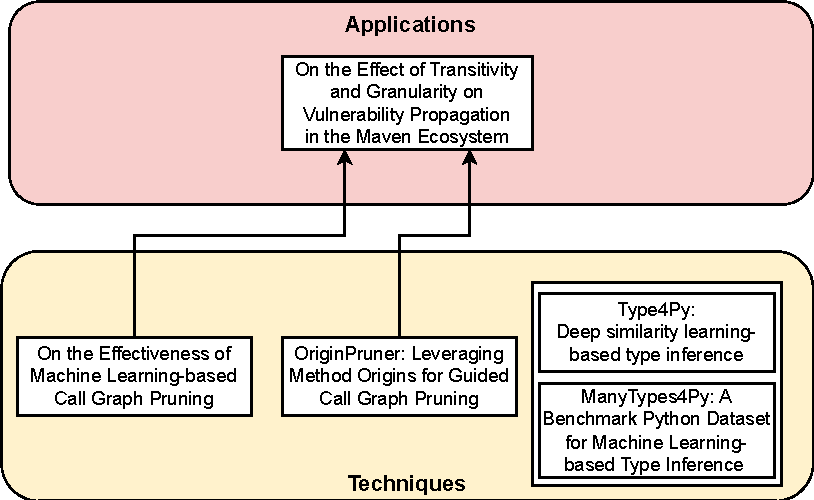
\includegraphics[width=\linewidth]{introduction/figs/thesis_overview.pdf}
 \caption{Overview of this PhD thesis.}
 \label{intro:fig:overall}
\end{figure}

\begin{itemize}
     \item In Chapter~\ref{ch:effect_ml_cg_pruning}, we addressed the RQ1 and conducted an empirical study on the effectiveness of ML-based call graph pruning. We addressed the limitations of previous research, such as a lack of a benchmark dataset, imbalanced training data, and reduced recall, which impacts practical downstream applications. To overcome these challenges, the study introduces the NYXCorpus, a new dataset comprising real-world Java programs with comprehensive test coverage. Our work also explores conservative pruning strategies during both the training and inference phases of ML-based CG pruners to improve the balance between recall and precision. Findings reveal the inherent difficulties of CG pruning in real-world Java projects, showing substantial improvements in precision at the cost of reduced recall. Despite these challenges, pruned CGs demonstrate comparable quality to those produced by context-sensitive 1-CFA analysis but are significantly smaller and faster to generate, offering nearly identical outcomes in downstream analyses. Using the proposed conservative strategies, ML-based CG pruning can achieve a more efficient balance between precision and recall, thereby enhancing the utility of static CGs in practical downstream applications.
    
    \item In Chapter~\ref{ch:origin_pruner}, we also addressed RQ1 and presented \tool{OriginPruner}, a novel technique for pruning edges in static call graphs. Static CGs commonly face challenges like over-approximation, which compromises their utility by inflating their size and introducing imprecision. \tool{OriginPruner} leverages the concept of method origin, identifying methods that introduce a signature within a class hierarchy and are often overridden to prune false edges effectively. Additionally, by integrating localness analysis, which assesses the scope of method interactions, \tool{OriginPruner} can confidently identify and eliminate edges related to origin methods, thereby enhancing CG precision. Key findings show that specific dominant origin methods, such as \texttt{Iterator.next}, significantly influence CG sizes; the derivatives of such origin methods are predominantly local, allowing for their safe pruning without detrimentally impacting downstream inter-procedural analyses. Also, \tool{OriginPruner} can significantly reduce CG size while preserving the soundness required for security applications like vulnerability propagation analysis, and it achieves these improvements with minimal computational overhead. These findings imply that incorporating domain knowledge about the type system into CG pruning strategies offers a viable and promising path for enhancing the performance of static program analysis.
    
    \item In Chapter~\ref{ch:effect_trans_gran}, we addressed RQ2 and explored the application of call graphs in vulnerability analysis and studied the effect of transitivity and granularity on vulnerability propagation in the Maven ecosystem. Past studies assess vulnerability impact at the dependency level, which arguably overestimates the actual risk to projects. Focusing on the Maven ecosystem, we adopt a more granular approach by analyzing a dataset of 3 million recent Maven packages, including their full transitive dependencies, to construct call graphs and perform reachability analysis. This allows for a more accurate identification of genuinely at-risk Maven packages. The findings reveal that while a significant portion of packages appears vulnerable when considering all transitive dependencies, a small percentage have reachable paths to vulnerable code, indicating a lower risk than previously found. Also, limiting dependency tree depth could efficiently reduce the computational load of a granular analysis. The chapter concludes with implications for software engineering, highlighting the value of granular vulnerability assessments over simpler, dependency-level analyses, providing actionable insights for improving security practices in software development. 

    \item In Chapter~\ref{ch:t4py}, we addressed RQ3 and proposed \tool{Type4Py}, a deep similarity learning-based hierarchical neural network model. While enhancing developer flexibility and productivity, the lack of static typing in dynamic languages like Python can lead to runtime exceptions. Python's PEP 484 introduced optional type annotations as a means to address these issues. However, it is a daunting task to retrofit types into existing codebases manually. \tool{Type4Py} learns to distinguish between similar and dissimilar types in high-dimensional space, facilitating type inference through the nearest-neighbor search. Unlike the previous work, which relied on potentially unsound human-provided type annotations, \tool{Type4Py} is trained and evaluated on a type-checked dataset, offering a more reliable assessment of its practicality through mean reciprocal rank (MRR). Empirical results show that \tool{Type4Py} significantly outperforms state-of-the-art approaches, achieving a substantial increase in MRR, therefore indicating its effectiveness in inferring type annotations. Additionally, the chapter discusses the development of a Visual Studio Code extension that employs \tool{Type4Py} to assist developers with ML-based type auto-completion for Python, further aiding in retrofitting types into existing codebases and enhancing productivity and code quality. \tool{Type4Py}'s inferred types can be used to aid applications like call graph construction and unit test generation for Python. In this thesis, we have not explored these applications. 
\end{itemize}

Also, Table~\ref{tab:chap-methods} shows research methods used in each chapter.

\begin{table}[ht]
\centering
\resizebox{\textwidth}{!}{\begin{tabular}{@{}lccc@{}}
\toprule
\textbf{Chapter} & \textbf{Mining Software Repositories} & \textbf{Training ML Models} & \textbf{Performance Evaluation} \\ \midrule
Chapter~\ref{ch:effect_ml_cg_pruning} & \checkmark & \checkmark & \checkmark \\ 
Chapter~\ref{ch:origin_pruner} & \checkmark & & \checkmark \\ 
Chapter~\ref{ch:effect_trans_gran} & \checkmark &  &  \\ 
Chapter~\ref{ch:t4py} & \checkmark & \checkmark & \checkmark \\ \bottomrule
\end{tabular}}
\caption{Chapters and the research method used}
\label{tab:chap-methods}
\end{table}

% \section{Thesis Contributions}
% This thesis presents several novel contributions aiming at enhancing software analysis tasks such as type inference and call graph pruning using machine learning.

% \begin{itemize}
%     \item We conducted an empirical study on the effectiveness of ML-based call graph pruning. We created the NYXCorpus dataset to evaluate ML-based call graph pruners. Also, we proposed conservative strategies to improve soundness or recall after CG pruning. Our empirical results show the efficacy of our proposed conservative strategy for the vulnerability propagation analysis, i.e., faster analysis time and tiny loss in soundness.

%     \item We proposed \tool{OriginPruner}, a novel approach for pruning edges in static call graphs. To prune false edges, the proposed approach is based on the concept of method origin and localness analysis. The experimental results show that \tool{OriginPruner} effectively makes CGs smaller while maintaining the soundness required for the vulnerability analysis. 

%     \item We conducted an empirical study on the effect of transitivity and granularity on vulnerability propagation in
% the Maven ecosystem. For this study, we employed both dependency- and method-level analysis to study security vulnerabilities in 3 million Maven packages. Our empirical findings reveal that a method-level analysis provides more accurate vulnerability assessments compared to a naive dependency-level analysis.

%     \item Finally, we proposed \tool{Type4Py}, a deep similarity learning-based hierarchical neural network model to infer type annotations for Python. Specifically, the proposed model learns to distinguish between similar and dissimilar types in high-dimensional space, namely, \textit{type clusters}. For evaluating ML-based type inference tools, we also proposed a benchmark dataset, ManyTypes4Py~\cite{mt4py2021}. The experimental results show \tool{Type4Py} outperforms the state-of-the-art ML-based type inference approaches and is effective at assisting developers to retrofit type annotations to their Python codebases.

% \end{itemize}

\section{Origins of Chapters}
Except for Chapter~\ref{ch:origin_pruner} currently under submission, all chapters of this thesis have been published in software engineering conferences (ICSE, MSR, and SANER). Each chapter of this thesis is self-contained and has its introduction, related work, and evaluation.

\begin{itemize}
    \item \textbf{Chapter}~\ref{ch:effect_ml_cg_pruning} is based on the published paper On the Effectiveness of Machine Learning-based Call Graph Pruning: An Empirical Study by Amir M. Mir, Mehdi Keshani, and Sebastian Proksch at the 21st International Conference on Mining Software Repositories (MSR) 2024.

    \item \textbf{Chapter}~\ref{ch:origin_pruner} is based on the paper OriginPruner: Leveraging Method Origins for Guided Call Graph Pruning by Amir M. Mir, Mehdi Keshani, and Sebastian Proksch. We are planning to submit this work to a software engineering conference by the end of 2024.

    \item \textbf{Chapter}~\ref{ch:effect_trans_gran} is based on the published paper On the Effect of Transitivity and Granularity on Vulnerability Propagation in the Maven Ecosystem by Amir M. Mir, Mehdi Keshani, and Sebastian Proksch at IEEE International
Conference on Software Analysis, Evolution and Reengineering (SANER) 2023.

    \item \textbf{Chapter}~\ref{ch:t4py} is based on the published paper Type4Py: Practical Deep Similarity Learning-Based Type Inference for Python by Amir M. Mir, Evaldas Latoškinas, Sebastian Proksch, and Georgios Gousios at the 44th International Conference on Software Engineering (ICSE) 2022. Also, the \tool{Type4Py} model was trained and evaluated on the published dataset paper ManyTypes4Py: A Benchmark Python Dataset for Machine Learning-based Type Inference by Amir M. Mir, Evaldas Latoškinas, and Georgios Gousios at the 18th International Conference on Mining Software Repositories (MSR) 2022.
\end{itemize}

